We ran 10 trials of each configuration. Since some tests failed, we had to
remove some data, so we were left with less trials per condition. The exact
number of trials can be found in \autoref{tab:trial}.

\subsection{Experimental findings}

\begin{table}
    \centering
    \caption{Number of trials for each condition}
    \label{tab:trial}
    \begin{tabular}{l|ccc}
        Rescue bots & 1 & 3 & 3 \\
        Search bots & 1 & 3 & 6 \\ \hline
        Mothership  & 7 & 8 & 9 \\
        Supervisor  & 7 & 6 & 7
    \end{tabular}
\end{table}

The result of our experiment can be found in \autoref{fig:barplot}. In the
figure can be seen that there is no difference in mean rescue time between
the mothership and the supervisor in any of our three conditions. We can
also see that there is no difference between the conditions with 3 or 6
searching agents. There is a difference between the 1 searching agent and 1
rescuing agent versus the other two conditions, which can be explained by
the lack of manpower in that condition. 

\begin{figure}
    \centering
    \resizebox{0.75\textwidth}{!}{
        % Created by tikzDevice version 0.8.1 on 2015-10-21 22:38:45
% !TEX encoding = UTF-8 Unicode
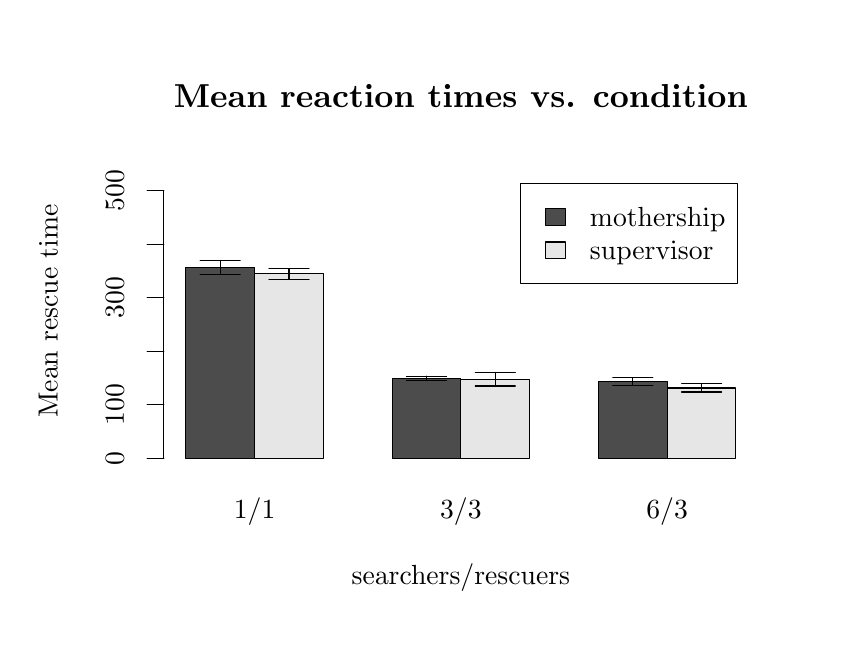
\begin{tikzpicture}[x=1pt,y=1pt]
\definecolor{fillColor}{RGB}{255,255,255}
\path[use as bounding box,fill=fillColor,fill opacity=0.00] (0,0) rectangle (289.08,216.81);
\begin{scope}
\path[clip] (  0.00,  0.00) rectangle (289.08,216.81);
\definecolor{drawColor}{RGB}{0,0,0}
\definecolor{fillColor}{gray}{0.30}

\path[draw=drawColor,line width= 0.4pt,line join=round,line cap=round,fill=fillColor] ( 57.15, 61.20) rectangle ( 82.00,130.17);
\definecolor{fillColor}{RGB}{230,230,230}

\path[draw=drawColor,line width= 0.4pt,line join=round,line cap=round,fill=fillColor] ( 82.00, 61.20) rectangle (106.85,127.84);
\definecolor{fillColor}{gray}{0.30}

\path[draw=drawColor,line width= 0.4pt,line join=round,line cap=round,fill=fillColor] (131.69, 61.20) rectangle (156.54, 90.09);
\definecolor{fillColor}{RGB}{230,230,230}

\path[draw=drawColor,line width= 0.4pt,line join=round,line cap=round,fill=fillColor] (156.54, 61.20) rectangle (181.39, 89.78);
\definecolor{fillColor}{gray}{0.30}

\path[draw=drawColor,line width= 0.4pt,line join=round,line cap=round,fill=fillColor] (206.23, 61.20) rectangle (231.08, 88.94);
\definecolor{fillColor}{RGB}{230,230,230}

\path[draw=drawColor,line width= 0.4pt,line join=round,line cap=round,fill=fillColor] (231.08, 61.20) rectangle (255.93, 86.62);
\end{scope}
\begin{scope}
\path[clip] (  0.00,  0.00) rectangle (289.08,216.81);
\definecolor{drawColor}{RGB}{0,0,0}

\node[text=drawColor,anchor=base,inner sep=0pt, outer sep=0pt, scale=  1.00] at ( 82.00, 39.60) {1/1};

\node[text=drawColor,anchor=base,inner sep=0pt, outer sep=0pt, scale=  1.00] at (156.54, 39.60) {3/3};

\node[text=drawColor,anchor=base,inner sep=0pt, outer sep=0pt, scale=  1.00] at (231.08, 39.60) {6/3};
\end{scope}
\begin{scope}
\path[clip] (  0.00,  0.00) rectangle (289.08,216.81);
\definecolor{drawColor}{RGB}{0,0,0}

\path[draw=drawColor,line width= 0.4pt,line join=round,line cap=round] (177.99,160.38) rectangle (256.65,124.38);
\definecolor{fillColor}{gray}{0.30}

\path[draw=drawColor,line width= 0.4pt,line join=round,line cap=round,fill=fillColor] (186.99,151.38) rectangle (194.19,145.38);
\definecolor{fillColor}{RGB}{230,230,230}

\path[draw=drawColor,line width= 0.4pt,line join=round,line cap=round,fill=fillColor] (186.99,139.38) rectangle (194.19,133.38);

\node[text=drawColor,anchor=base west,inner sep=0pt, outer sep=0pt, scale=  1.00] at (203.19,144.94) {mothership};

\node[text=drawColor,anchor=base west,inner sep=0pt, outer sep=0pt, scale=  1.00] at (203.19,132.94) {supervisor};

\node[text=drawColor,anchor=base,inner sep=0pt, outer sep=0pt, scale=  1.20] at (156.54,188.07) {\bfseries Mean reaction times vs. condition};

\node[text=drawColor,anchor=base,inner sep=0pt, outer sep=0pt, scale=  1.00] at (156.54, 15.60) {searchers/rescuers};

\node[text=drawColor,rotate= 90.00,anchor=base,inner sep=0pt, outer sep=0pt, scale=  1.00] at ( 10.80,114.41) {Mean rescue time};
\end{scope}
\begin{scope}
\path[clip] (  0.00,  0.00) rectangle (289.08,216.81);
\definecolor{drawColor}{RGB}{0,0,0}

\path[draw=drawColor,line width= 0.4pt,line join=round,line cap=round] ( 49.20, 61.20) -- ( 49.20,157.94);

\path[draw=drawColor,line width= 0.4pt,line join=round,line cap=round] ( 49.20, 61.20) -- ( 43.20, 61.20);

\path[draw=drawColor,line width= 0.4pt,line join=round,line cap=round] ( 49.20, 80.55) -- ( 43.20, 80.55);

\path[draw=drawColor,line width= 0.4pt,line join=round,line cap=round] ( 49.20, 99.89) -- ( 43.20, 99.89);

\path[draw=drawColor,line width= 0.4pt,line join=round,line cap=round] ( 49.20,119.24) -- ( 43.20,119.24);

\path[draw=drawColor,line width= 0.4pt,line join=round,line cap=round] ( 49.20,138.59) -- ( 43.20,138.59);

\path[draw=drawColor,line width= 0.4pt,line join=round,line cap=round] ( 49.20,157.94) -- ( 43.20,157.94);

\node[text=drawColor,rotate= 90.00,anchor=base,inner sep=0pt, outer sep=0pt, scale=  1.00] at ( 34.80, 61.20) {0};

\node[text=drawColor,rotate= 90.00,anchor=base,inner sep=0pt, outer sep=0pt, scale=  1.00] at ( 34.80, 80.55) {100};

\node[text=drawColor,rotate= 90.00,anchor=base,inner sep=0pt, outer sep=0pt, scale=  1.00] at ( 34.80,119.24) {300};

\node[text=drawColor,rotate= 90.00,anchor=base,inner sep=0pt, outer sep=0pt, scale=  1.00] at ( 34.80,157.94) {500};
\end{scope}
\begin{scope}
\path[clip] ( 49.20, 61.20) rectangle (263.88,167.61);
\definecolor{drawColor}{RGB}{0,0,0}

\path[draw=drawColor,line width= 0.4pt,line join=round,line cap=round] ( 69.57,127.60) -- ( 69.57,132.74);

\path[draw=drawColor,line width= 0.4pt,line join=round,line cap=round] ( 62.35,127.60) --
	( 69.57,127.60) --
	( 76.80,127.60);

\path[draw=drawColor,line width= 0.4pt,line join=round,line cap=round] ( 76.80,132.74) --
	( 69.57,132.74) --
	( 62.35,132.74);

\path[draw=drawColor,line width= 0.4pt,line join=round,line cap=round] ( 94.42,125.95) -- ( 94.42,129.73);

\path[draw=drawColor,line width= 0.4pt,line join=round,line cap=round] ( 87.19,125.95) --
	( 94.42,125.95) --
	(101.65,125.95);

\path[draw=drawColor,line width= 0.4pt,line join=round,line cap=round] (101.65,129.73) --
	( 94.42,129.73) --
	( 87.19,129.73);

\path[draw=drawColor,line width= 0.4pt,line join=round,line cap=round] (144.12, 89.26) -- (144.12, 90.91);

\path[draw=drawColor,line width= 0.4pt,line join=round,line cap=round] (136.89, 89.26) --
	(144.12, 89.26) --
	(151.34, 89.26);

\path[draw=drawColor,line width= 0.4pt,line join=round,line cap=round] (151.34, 90.91) --
	(144.12, 90.91) --
	(136.89, 90.91);

\path[draw=drawColor,line width= 0.4pt,line join=round,line cap=round] (168.96, 87.34) -- (168.96, 92.22);

\path[draw=drawColor,line width= 0.4pt,line join=round,line cap=round] (161.74, 87.34) --
	(168.96, 87.34) --
	(176.19, 87.34);

\path[draw=drawColor,line width= 0.4pt,line join=round,line cap=round] (176.19, 92.22) --
	(168.96, 92.22) --
	(161.74, 92.22);

\path[draw=drawColor,line width= 0.4pt,line join=round,line cap=round] (218.66, 87.65) -- (218.66, 90.24);

\path[draw=drawColor,line width= 0.4pt,line join=round,line cap=round] (211.43, 87.65) --
	(218.66, 87.65) --
	(225.89, 87.65);

\path[draw=drawColor,line width= 0.4pt,line join=round,line cap=round] (225.89, 90.24) --
	(218.66, 90.24) --
	(211.43, 90.24);

\path[draw=drawColor,line width= 0.4pt,line join=round,line cap=round] (243.51, 85.15) -- (243.51, 88.09);

\path[draw=drawColor,line width= 0.4pt,line join=round,line cap=round] (236.28, 85.15) --
	(243.51, 85.15) --
	(250.73, 85.15);

\path[draw=drawColor,line width= 0.4pt,line join=round,line cap=round] (250.73, 88.09) --
	(243.51, 88.09) --
	(236.28, 88.09);
\end{scope}
\end{tikzpicture}
}
    \caption{The mean rescue time for the mothership and the supervisor
        versus the different conditions. The error bars on the plot show
        the standard error}
    \label{fig:barplot}
\end{figure}

\subsection{Interpretation}
From these results we can conclude that there is no difference between our
two implementations of the central brain. We expect this is because the
central brains both use the same strategy, and that strategy is not the
optimal strategy for this problem. This means that there are other
bottlenecks in both implementations that slow the simulation down more
than the communication between the agents. 

Another explanation for why we didn't see this effect might be that during our
testing we did not stress the system enough. This means we should repeat
the experiment with a heavier load and see if that changes the results.
However, on our current test machine, running that simulation would take to
much time. 
